\documentclass[12pt]{article}
\usepackage{hyperref}
\usepackage[a4paper]{geometry}
\usepackage{graphicx}
\usepackage{listings}
\usepackage{multirow}

\newcommand{\fitxategi}[1] {\underline{\textit{#1}}}
\newcommand{\metodo}[1] {\textit{#1}}
\newcommand{\aldagai}[1] {\textit{#1}}
\newcommand{\tekla}[1] {\textbf{#1}}
\newcommand{\erref}[1] {\textbf{\ref{#1}}}

\renewcommand{\contentsname}{Edukiak}
\renewcommand{\refname}{Erreferentziak}


\geometry{
 a4paper,
 total={170mm,257mm},
 left=2cm,
 top=2cm,
 }


\title{KbG proiektua: 3. fasea}
\author{
        Oier Irazabal\\
        Jesus Calleja
}
\date{\today}



\begin{document}
\maketitle

%\begin{abstract}
%This is the paper's abstract \ldots
%\end{abstract}

\tableofcontents

\vspace{2cm}
\begin{center}
%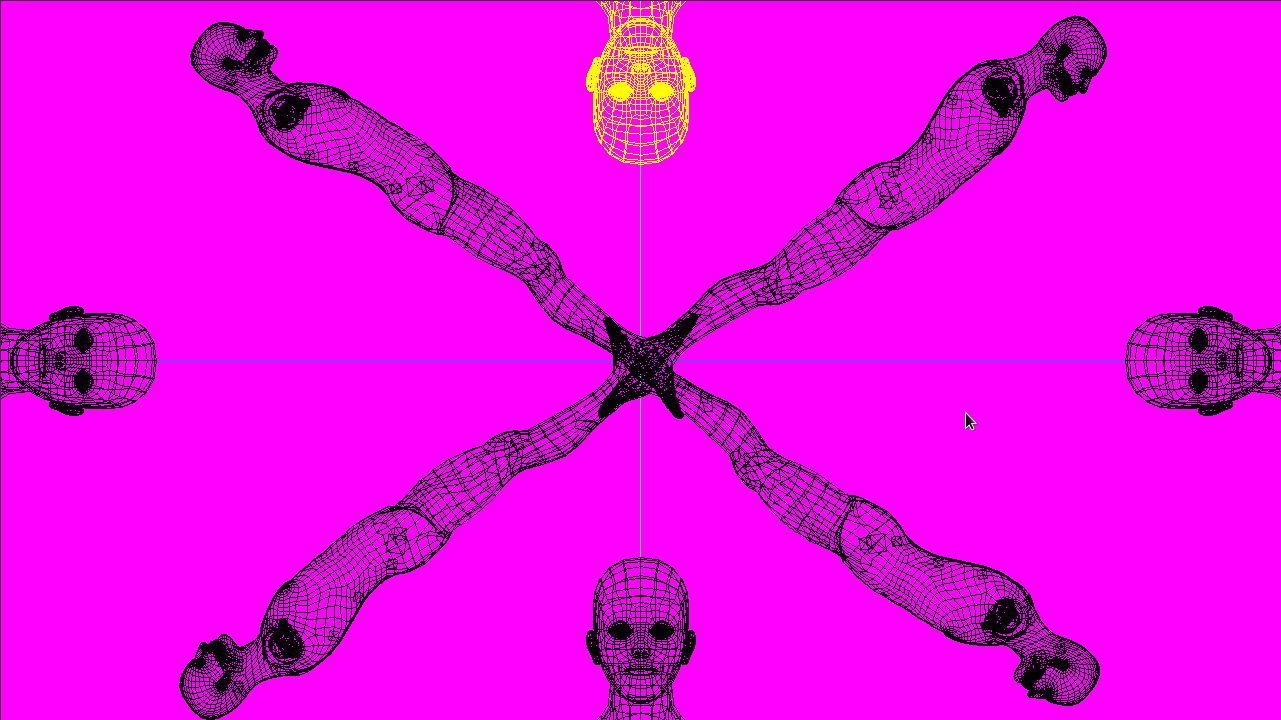
\includegraphics[scale=0.35]{kaizo.png}\\
\end{center}

\pagebreak

\section{Kamera}

Fase honetan lortutako inplementazioa bi kamera motaren txertaketa izan da. Orain arte ingurunearen ikuspegi finko eta ez-fidela genuen. Proiekzioa ortografikoa zen; hau da, argi-izpiak Z ardatzarekiko paraleloak ziren, sakoneraren nozioa galduz. Gainera, kamera jatorrian geldi zegoen, objektuak izanik mugitu ZIRENTEKETEN bakarrak.\\

Orain, bi kamera mota berri aukera daitezke: libreki mugi daitekeen perspektibazkoa, eta ibiltaria. \tekla{C} tekla sakatuz gero, kamera-motaz aldatzen da. Kamera hautatzeko gai izateaz gain, kamera transformatu ahal izateko, \tekla{K} tekla sakatzea dago, aukeratutako transformazioa kamerari aplikatzeko eta ez objektuari. Aitzitik, objektuak transformatzeko berriz, \tekla{O} tekla sakatu behar da.\\

Ideia teorikoak finkatu ditugu, baina nola lor daitezke orain arte aipatutako emaitza guztiak? Zerk osatzen du kamera bat?
Alde batetik, zein kamera motarekin ari garen hartu behar da kontutan, bestetik proiekzio motaz aldatu behar da hautatutako kameraren arabera, eta azkenik kameraren mugimendua eta biraketa simulatu behar dira. Horretarako hurrengo datu-egitura erabiliko dugu:

\begin{center}
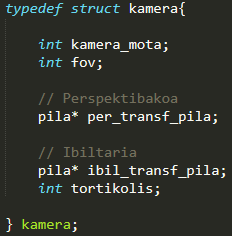
\includegraphics[scale=1]{kamera_struct.png}

\textbf{1. irudia}: kamera datu-egitura
\end{center}


Egiturako kideen azalpenak:

\begin{itemize}
\item \aldagai{kamera\_mota}: kamera ortografikoa, perspektibazkoa edo ibiltaria den adierazten du (ikus \erref{constants} atala)
\item \aldagai{fov}: Field Of View\cite{fov}, \erref{per_proj} atalean azaldua.
\item \aldagai{per\_transf\_pila}: perspektibazko kamera transformatzeko erabiltzen den aldaketa-pila, \erref{kam_sim} atalean azaldua.
\item \aldagai{ibil\_transf\_pila}: kamera ibiltaria transformatzeko erabiltzen den aldaketa-pila, \erref{kam_sim} atalean azaldua.
\item \aldagai{tortikolis}: kamera ibiltariak plano horizontalarekiko daukan angeluarekiko proportzionala den balio bat. Bertikalki bira daitekeen eremua mugatzeko balio du.
\end{itemize}

\textbf{Oharra}: pila hauek objektuek erabiltzen dutenaren bera dira.\\

Kamerarekin zerikusia duten metodo edo egitura guztiak \fitxategi{kamera.c} eta \fitxategi{kamera.h} fitxategietan daude.
Bestalde, \textbf{\_k} aldagaia \fitxategi{main.c} fitxategian definitzen eta hasieratzen da aldagai global bezala, kamera bakar bat erabiltzen duelako aplikazioak oraingoz.


\subsection{Perspektibazko proiekzioa}\label{per_proj}
Orain arte \fitxategi{display.c} fitxategiko \metodo{display()} metodoan, \metodo{glOrtho()} metodoa erabiltzen genuen proiekzio ortografikoa lortzeko. Hala ere, orain txertatutako beste bi kamera motek ez dute proiekzio bera erabiltzen, perspektibazkoa baizik. Beraz, proiekzio mota kamera motaren menpe geratuko da eta kamera ortografikoaz beste, \metodo{gluPerspective()}\cite{glu_perspective} izaneko metodoa erabiliko dugu proiekzio mota berria lortzeko.\\
Hona hemen pausu hau azaltzeko sasikodea:

\begin{center}
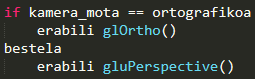
\includegraphics[scale=1]{kamera_projection.png}

\textbf{2. irudia}: Proiekzioa burutzeko sasikodea
\end{center}

Metodo berri honek lau argumentu hartzen ditu: \textit{FOV}, leihoaren aspektuaren erlazioa (aspect ratio)\cite{aspect_ratio} eta \textit{near} eta \textit{far} Z-planoak\cite{near_far}. Lau argumentuek \textit{frustum}\cite{frustum} izeneko bistaratze-eremua mugatuko dute. Irudi honek erakusten du \textit{frustum}-a nola mugatzen duten parametroek:

\begin{center}
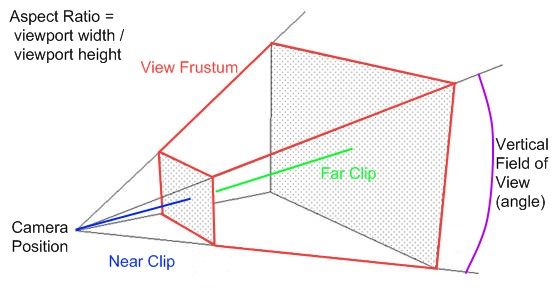
\includegraphics[scale=0.8]{kamera_frustum.jpg}

\textbf{3. irudia}: Kameraren \textit{frustum}-a
\end{center}

AZALDU PARAMETROAK\\

\textit{near} eta \textit{far} planoaren balioak eta \textit{FOV}-aren hasierako balioa, minimoa eta maximoa \fitxategi{definitions.h} fitxategian definituta daude, lehenengo biak konstateak izanik (ikus \erref{constants} atala). \textit{FOV}-a kontrolatzeko kameraren egiturako \aldagai{fov} kidea erabiltzen da. Aldagai honek kamerak zenbat ikus dezakeen kontrolatzen duenez, zoom egitea ahalbidetzen digu kamera ortografikoaren moduan (\tekla{CTRL +} eta \tekla{CTRL -} teklen konbinaketekin). Azkenik, aspektuaren erlazioa \fitxategi{display.c} fitxategiko \metodo{reshape()} metodoak kontrolatzen du, leihoaren dimentsioak aldatzea posible baita. Balioa \aldagai{\_window\_ratio} aldagai globalean gordetzen da.


\subsection{Kameraren efektua}\label{kam_sim}

Transformazioak objektuei aplikatzen zaizkie. Kontraesana dirudien arren, izatez kameraren kontzeptua ez da existitzen ordenagailu bidezko grafikoetan. Kamera ezkerretara mugitzea simulatu nahi izanez gero, mundu guztia eskuinetarantz mugitu beharko da proportzio berean, ilusio hori lortzeko. Hau esanda, ondoriozta daiteke kamera simulatzeko objektu guztien transformazioa kargatu baino lehen kamerarena kargatu beharko dela.

\begin{center}
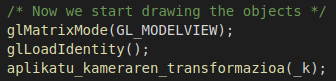
\includegraphics[scale=1]{kamera_transform.png}

\textbf{4. irudia}: kameraren transformazioaren aplikazioa
\end{center}

\textbf{Oharra}: Objektuak marrazteko begiztaren amaieran, identitate matrizea kargatu ostean, berriro aplikatu behar da kameraren transformazioa.\\

Kameraren transformazioa burutzeko \metodo{gluLookAt()}\cite{glu_lookat} metodoa erabiltzen dugu. Funtzio honek kameraren posizioa, begira dagoen puntuaren posizioa eta goranzko norabidea adierazten duen bektorea emanik, uneko matrizea (gure kasuan MODELVIEW) aldatzen du kameraren transformazioa simulatzeko. Datu hauek lortzeko, hasierako \aldagai{eye}, \aldagai{look} eta \aldagai{up} balioak (\metodo{gluLookAt()} funtzioaren parametroak hurrenez hurren) finkatuko ditugu, eta horien aldaketak ahalbidetzeko transformazio-matrizeen pila bat erabiliko dugu, non hasierako aldagaiak transformazioarekin biderkatuta, kameraren uneko posizioa eta errotazioa kalkulatu ahalko dugun. HOBETO ESPLIKE BIKO DA IGUAL. ZUZENDU UP EZ IZETIE POINT3, VECTOR3 BAIO!

\begin{center}
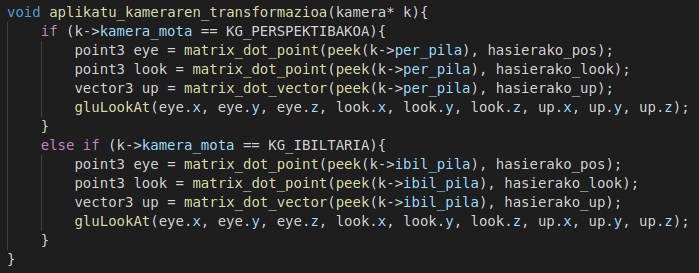
\includegraphics[scale=0.8]{kamera_lookat.png}

\textbf{5. irudia}: \metodo{gluLookAt()}-en erabilpena
\end{center}

\begin{center}
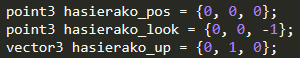
\includegraphics[scale=1]{kamera_hasierako_balioak.png}

\textbf{6. irudia}: hasierako balioak
\end{center}

Kalkuluak egiteko erabilitako bi biderketen metodoak \erref{transformazioak}. atalean daude azalduta.


\subsection{Perspektibazko kamera}

Kamera hau libreki mugi eta bira daiteke espazioan, oso erabilgarria izanik ingurunea ikuspuntu askotatik aztertu ahal izateko. Adibidez, Blender\cite{blender} eta itxura horretako aplikazioek aukera hau eskaintzen dute.

\subsubsection{Transformazioak}

Kamerak translatzeko eta biratzeko aukera du, eskalatzea eta zizailatzeak zentzurik ez baitaukate. Bi aldaketa hauek lokalean zein globalean egin daitezke. Mugimendua globala denean, munduko X, Y eta Z ardatzetan emango da translazioa, lokalean aldiz, uneko begiradaren norabidearen araberakoa izango da. Biraketa globala denean, kamerak jatorriaren inguruan biratuko du hautatutako ardatzean, lokalean aldiz, kamera geldi geratuko da, begiradaren norabidea aldatuz.\\

OINARTE EINDDOT, HAMENDIK BERA GEHIXEN BAT ZE AZALDU DINOEN NOTATXUEK DIE:\\

mobidu, lokal zein global, azaldu bixek

gireu global origenan ingeruen edo lokal kamarie geldi ta giretan.

beste transformak ezteke zentzurik

\subsection{Kamera ibiltaria}

Pertsona bat simuletan daben kamarie. Lurrera inketa dau.

\subsubsection{Transformazioak}

Diferentie, ezta mobitzen ta rotetan ardatz danatak ta global ta lokalien.

Bakarrik eurrea ta atzea mobidulei. Mobidu ezker-eskuma ta gora-bera baia hau azkena limiteta dau.

Zelan lortzen da lurrera inketa egotie? Ba ezker-eskumagaz eztau arazorik, baia gora-bera beittutetakoan ta mobitzerakoan, kalkuletan da ze alturan geratuko zna ta transform global bat eitten da Y ardatzien kontrara kontrarrestetako ta lurrien inketa geatzeko.

\subsection{Aldaketak desegitea eta berregitea}

INTRODUCIDU ALDAKETAK EITTIE ZER DAN, PILA BAT ZEAITTIK ETAB... BAIA EZ ESAN ZELAN DAUEN INPLEMENTETA

Objektuekin bezala, kamerari aplikatutako transformazioak desegitea eta berregitea badago, pila mota berdinak baitira. Kamera mota bakoitza bata-bestearekiko independentea izatea nahi dugunez, perspektibazko kamerarentzako pila bat eta ibiltariarentzako beste bat sortuko ditugu (ikus 1. irudia). Demagun perspektibazko kamerari edozein hiru transformazio lokal aplikatzen dioguzela, orduan pilaren egoera hurrengoa izango zen:\\
transformazioen ordena lehenik \textbf{M1}, gero \textbf{M2} eta azkenik \textbf{M3} izanik eta \textbf{I} identitate matrizea,

\begin{center}
\begin{tabular}{r|r|r}
 \cline{2-2}
 $top \rightarrow$ & $\textbf{M3} \cdot \textbf{M2} \cdot \textbf{M1}$ & \\
 \cline{2-2}
 & $\textbf{M2} \cdot \textbf{M1}$ & \\
 \cline{2-2}
 & $\textbf{M1}$ & \hspace{0.5cm} ($\textbf{M1} \cdot \textbf{I} = \textbf{M1}$) \\
 \cline{2-2}
 & $\textbf{I}$ & \\
 \cline{2-2}
\end{tabular}

\textbf{1. diagrama}: Pilaren erabilpena.
\end{center}

Pilaren erabilera lau ekintzetan banatzen da:

\begin{itemize}
\item \textbf{Pila sortzea}. Identitate matrizea gordetzen duen pila bat itzultzen du \metodo{pila\_sortu()} metodoa erabiliz.

\item \textbf{Pilaratzea}. Matrize berri bat pilaratzen du. Orokorrean matrize hau aurreko matrizearen transformazio bat izango da, \metodo{peek()} (pilaren gaineko matrizea lortzeko) eta \metodo{push} (matrizea pilaratzeko) konbinatuz.

\item \textbf{Aldaketak desegitea}. Metodo honek azkenengo matrizea apuntatzen duen \textit{pointer}-a\cite{pointer} aurreko matrizera mugitzen du azkenengo posizioko elementua ezabatu gabe, azken aurreko aldaketa erakutsiz. Ekintza hau \metodo{pop()} metodoak burutzen du.

\item \textbf{Aldaketak berregitea}. Aurreko ekintzaren kontrakoa da, \textit{pointer}-a elementu bat aurrerago eramanez, \metodo{depop()} metodoak burutzen duena. 
\end{itemize}

Funtsean, pila bi zentzutara lotutako lista estekatu bat da. Datu egitura honek bi propietate garrantzitsu ematen dizkigu: pila nahi beste hazi ahal izatea (memoriarik gabe geratu arte) eta bi noranzko nabigagarritasuna, pilaren azken elementua bi aldeetara mugitzea ahalbidetzen duena (\metodo{pop()} eta \metodo{depop()}).\\
Hona hemen datu-egituraren diagrama bat:

\begin{center}

\fbox{\textbf{I}} $\leftrightarrow$ \fbox{\textbf{M1}} $\leftrightarrow$ \fbox{\textbf{M2} $\cdot$ \textbf{M1}} $\leftrightarrow$ \fbox{\textbf{M3} $\cdot$ \textbf{M2} $\cdot$ \textbf{M1}}

\hspace{5.5cm} $\uparrow$

\hspace{5.5cm} top

\textbf{2. diagrama}: Pilaren elementuen arteko lotura.
\end{center}


\section{transformazioak.c}\label{transformazioak}

oin klase batera mobidugu transformazinoakaz relacioneta dauena. bebai matriziek matriziekaz, puntoakaz ta bektorakaz biderkatzeko metodoak.


\section{Konstante berriak}\label{constants}

Sartuniko konstantiek kamarientzako die bakarrik.

ortografikoa, ...

aldaketak ia objetoari ala kamarieri

hasierako fov, near ta far planoak

kamara motie

...

\bibliographystyle{abbrv}
\bibliography{main}

\begin{thebibliography}{9}

\bibitem{glutSpecialFunc} 
\underline{glutSpecialFunc()}:\\
\url{https://www.opengl.org/resources/libraries/glut/spec3/node54.html}

% KENDU HAU (ARINAUKO REFERNTZIXE) TA SARTU BARRIXEK MODU COPYPASTE EITTEN

\end{thebibliography}


\end{document}

